\newcommand\skipCaption[1]{
  \vspace*{-6mm}
  \caption{#1}
}

\newcommand\skipCaptionA[2]{
  \vspace*{-#1mm}
  \caption{#2}
}

\chapter{Resultaten}
\label{hoofdstuk:resultaten}
Dit hoofdstuk bespreekt de resultaten van de nieuwe $\symBSPsweep$ bomen.
In sectie \ref{h5:praktische-aspecten} worden een aantal praktische aspecten omtrent de testopstelling besproken zoals de scenes, de gebruikte parameterwaarden en het gebruikte computersysteem.
Daarna bespreken we de invloed van het aantal richtingen op de vorm (sectie \ref{h5-richtingen-bespreking}) en kwaliteit (sectie \ref{h5-richtingen-kwaliteit}) van de negen soorten $\symBSPsweep$ bomen.
De laatste sectie (sectie \ref{h5-vergelijken}) vergelijkt de beste $\symBSPsweep$ bomen met de bomen besproken in hoofdstuk \ref{hoofdstuk:voorgaand-werk}.

\section{Praktische aspecten}
\label{h5:praktische-aspecten}
Alle $\symBSP$ bomen zijn geïmplementeerd in het pbrt \cite{pbrt} framework zoals besproken in hoofdstuk \ref{hoofdstuk:implementatie}. 
Dit framework maakt geen gebruik van optimalisaties zoals SIMD instructies en de GPU. 
Hierdoor kan de kracht van de verschillende bomen objectief vergeleken worden.\\

Figuur \ref{fig:results-scenes} toont de gebruikte testscenes en tabel \ref{tab:results-statistics-scenes} toont informatie over deze scenes.
De Killeroo Been scene is een scene waarbij algemene $\symBSP$ bomen voordeel hebben ten opzichte van de $\symKd$ boom omwille van de complexe geometrie waarop is ingezoomd.
De drie andere scenes zijn realistische indoor scenes.
Alle scenes maken gebruik van de in pbrt ingebouwde Halton sampling met een specifiek aantal stralen per pixel (\textit{spp}).
De globale belichting wordt berekend via \textit{path tracing} waarbij steeds een maximale diepte van 5 gebruikt wordt, behalve bij de museum scene waar enkel directe belichting gebruikt wordt.\\

\begin{figure}
  \begin{subfigure}[t]{0.25\textwidth}
    \centering
    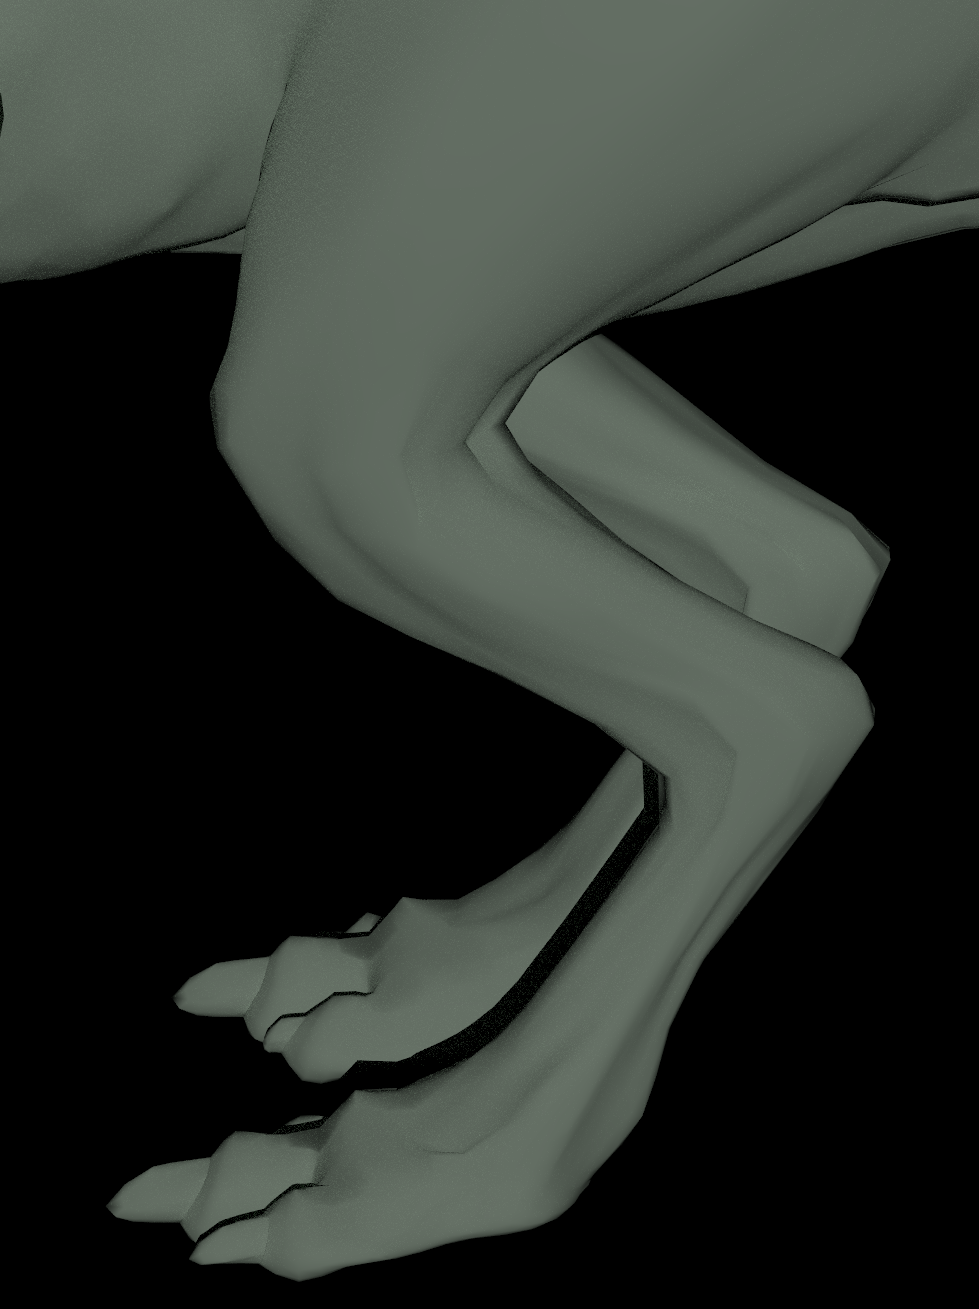
\includegraphics[width=0.6\linewidth]{img/killerooFeet}
    \caption{Killeroo Been scene}
    \label{fig:results-scene-killeroo-been}    
  \end{subfigure}
  \begin{subfigure}[t]{0.20\textwidth}
    \centering
    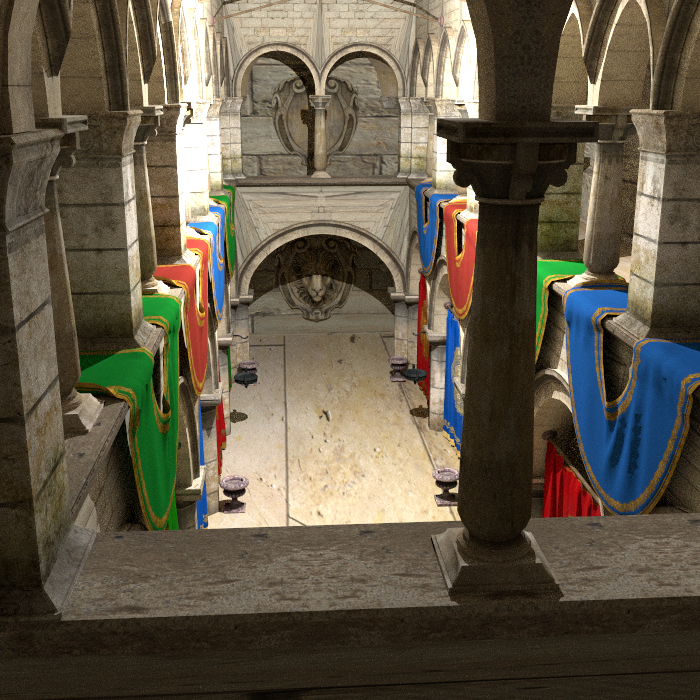
\includegraphics[width=1\linewidth]{img/sponza}
    \caption{Sponza scene}
    \label{fig:results-scene-sponza}    
  \end{subfigure}
  \begin{subfigure}[t]{0.29\textwidth}
    \centering
    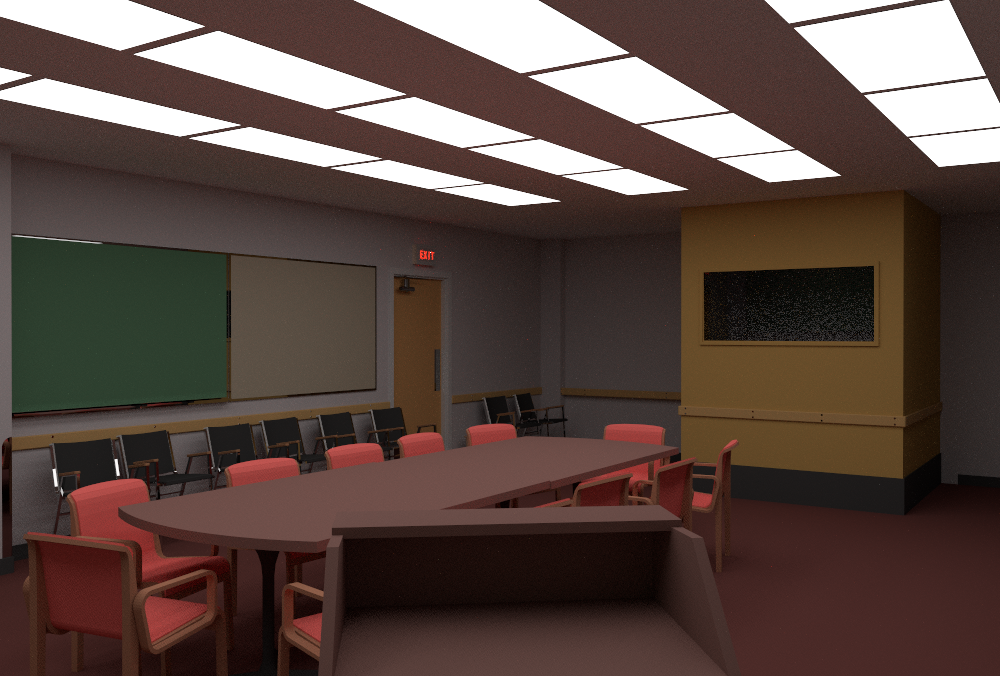
\includegraphics[width=1\linewidth]{img/conferencehall}
    \caption{Conference scene}
    \label{fig:results-scene-conference}    
  \end{subfigure}
  \begin{subfigure}[t]{0.20\textwidth}
    \centering
    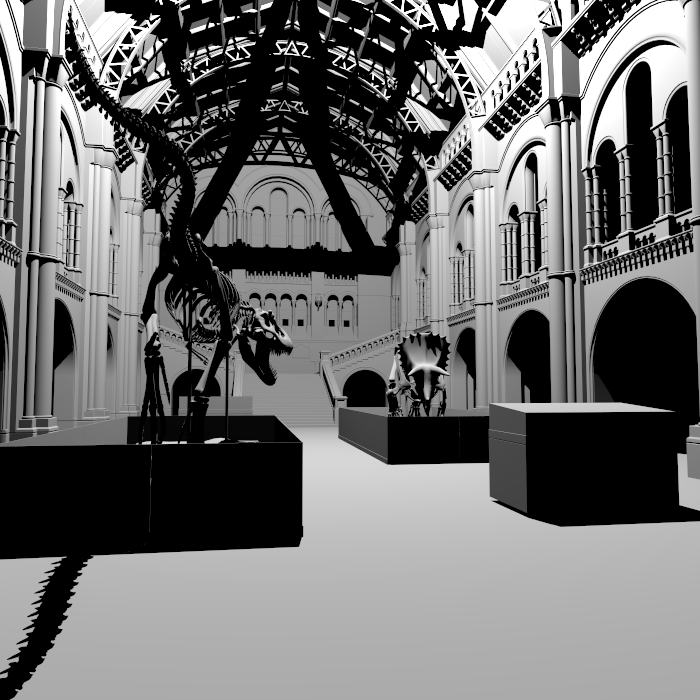
\includegraphics[width=1\linewidth]{img/museum}
    \caption{Museum scene}
    \label{fig:results-scene-museum}    
  \end{subfigure}
  \caption[Testscenes]{Testscenes - \small De testscenes gebruikt om de nieuwe $\symBSP$ te testen}
  \label{fig:results-scenes}
\end{figure}

\begin{table}
  \centering
  \begin{tabular}{@{}lcccc@{}} \toprule
  Scene & Aantal driehoeken & Resolutie & Sampling per pixel & Belichting\\ \midrule
  Killeroo Been & 33264 & 5000x5000 & Halton, 8spp & \textit{path tracing}, diepte 5\\
  Sponza & 227309 & 700x700 & Halton, 64spp & \textit{path tracing}, diepte 5\\
  Conference & 123651 & 1000x676 & Halton, 64spp & \textit{path tracing}, diepte 5\\
  Museum & 1462840 & 700X700 & Halton, 64spp & \textit{path tracing}, diepte 1\\ \bottomrule
 \end{tabular}
  \caption[Statistieken Testscenes]{Statistieken Testscenes - \small Statistieken van de testscenes gebruikt om de nieuwe $\symBSP$ bomen te testen}
  \label{tab:results-statistics-scenes}
\end{table}

Tabel \ref{tab:results-parameters} toont de parameterwaarden die gebruikt zijn bij de testen. De formule voor de maximale diepte is afhankelijk van het aantal driehoeken n en is bedacht door \authorHavranBittner{} \cite{havran2002improving} voor $\symKd$ bomen. Deze parameterwaarden zijn niet geoptimaliseerd en kunnen mogelijks beter worden afgesteld.
De specificaties van het gebruikte computersysteem worden getoond in figuur \ref{tab:results-specs}.
\begin{table}
  \centering
  \begin{tabular}{@{}lc@{}} \toprule
  Parameter & Waarde \\ \midrule
  $\symCost_\symIntersection$ & 80 \\
  $\symCostTraversalKd$ & 1 \\
  $\symCostTraversalBSP$ & 5 \\
  $\symMaxPrims$ & 1 \\
  $\symMaxDepth$ & $[k_1log_2(n) + k_2]$ met $k_1 = 1.6$ en $k_2 = 2$ \\
  $maxIteraties$ & 500 \\
  $\alpha$ & 0.1 \\
  \bottomrule
 \end{tabular}
  \caption[Gebruikte parameterwaarden]{Gebruikte parameterwaarden - \small De waarden van de parameters gebruikt bij het testen van de nieuwe $\symBSP$ bomen.}
  \label{tab:results-parameters}
\end{table}

\begin{table}
  \centering
  \begin{tabular}{@{}lc@{}} \toprule
  Parameter & Waarde \\ \midrule
  CPU & Intel Core i7-6700HQ CPU @ 2.60GHz x 8 \\
  Geheugen & 16 GB DDR4 \\
  Besturingssysteem & Ubuntu 18.04.2 LTS 64-bit \\
  \bottomrule
 \end{tabular}
  \caption[Specificaties computersysteem]{Specificaties computersysteem - \small De specificaties van het gebruikte computersysteem.}
  \label{tab:results-specs}
\end{table}

\newcommand{\plotVsK}[5] {
  \begin{tikzpicture}[scale=0.5]
    \begin{axis}[
      axis lines = left,
      ylabel = #5,
      xlabel = $k$,
      ymin=#3, ymax=#4,
      xmin=2,
      width=1.8\textwidth,
      height=2.2\textwidth,
      cycle multi list={%
        color list\nextlist
        [3 of]mark list
      },
      legend style={at={(0.5,-0.15)}, anchor=north,legend columns=3},
      title = #2,
  ]
    \addplot table [x=K, y=#1, col sep=comma] {data/bsprandomRender.csv};
    \addlegendentry{$\symBSPrandom$}
    \addplot table [x=K, y=#1, col sep=comma] {data/bsprandomwithkdRender.csv};
    \addlegendentry{$\symBSPrandomkd$}
    \addplot table [x=K, y=#1, col sep=comma] {data/bsprandomfastkdRender.csv};
    \addlegendentry{$\symBSPrandomfastkd$}
    
    \addplot table [x=K, y=#1, col sep=comma] {data/bsparbitraryRender.csv};
    \addlegendentry{$\symBSParbitrary$}
    \addplot table [x=K, y=#1, col sep=comma] {data/bsparbitrarywithkdRender.csv};
    \addlegendentry{$\symBSParbitrarykd$}
    \addplot table [x=K, y=#1, col sep=comma] {data/bsparbitraryfastkdRender.csv};
    \addlegendentry{$\symBSParbitraryfastkd$}
    
    \addplot table [x=K, y=#1, col sep=comma] {data/bspclusterRender.csv};
    \addlegendentry{$\symBSPcluster$}
    \addplot table [x=K, y=#1, col sep=comma] {data/bspclusterwithkdRender.csv};
    \addlegendentry{$\symBSPclusterkd$}
    \addplot table [x=K, y=#1, col sep=comma] {data/bspclusterfastkdRender.csv};
    \addlegendentry{$\symBSPclusterfastkd$}
      \end{axis}
    \end{tikzpicture}
}

\newcommand{\plotFastKdVsK}[5] {
  \begin{tikzpicture}[scale=0.5]
    \begin{axis}[
      axis lines = left,
      ylabel = #5,
      xlabel = $k$,
      ymin=#3, ymax=#4,
      width=1.8\textwidth,
      height=2.2\textwidth,
      cycle multi list={%
        color list\nextlist
        mark=triangle*
      },
      legend style={at={(0.5,-0.15)}, anchor=north,legend columns=3},
      title = #2,
  ]
    
    \addplot table [x=K, y=#1, col sep=comma, mark=diamond*] {data/bsprandomfastkdRender.csv};
    \addlegendentry{$\symBSPrandomfastkd$}
    
    \addplot table [x=K, y=#1, col sep=comma, mark=diamond*] {data/bsparbitraryfastkdRender.csv};
    \addlegendentry{$\symBSParbitraryfastkd$}
    
    \addplot table [x=K, y=#1, col sep=comma, mark=diamond*] {data/bspclusterfastkdRender.csv};
    \addlegendentry{$\symBSPclusterfastkd$}
      \end{axis}
    \end{tikzpicture}
}

\newcommand{\plotRendertimeKScenes}[4] {
  \begin{tikzpicture}
    \begin{axis}[
      axis lines = left,
      ylabel = Procentuele tijd tov de $\symKd$ boom,
      xlabel = $k$,
      ymin=#3, ymax=#4,
      width=0.5\textwidth,
      height=0.8\textwidth,
      %cycle multi list={%
      %  color list\nextlist
      %  [3 of]mark list
      %},
      title = #2,
      legend pos=north east,
  ]
    \addplot table [x=K, y=RendertimeTovKdFeet, col sep=comma] {#1};
    \addlegendentry{Med Killeroo Been}
    \addplot table [x=K, y=RendertimeTovKdSponza, col sep=comma] {#1};
    \addlegendentry{Med Sponza Been}
    \addplot table [x=K, y=RendertimeTovKdConference, col sep=comma] {#1};
    \addlegendentry{Med Conference Been}
    
      \end{axis}
    \end{tikzpicture}
}
\newcommand{\plotSAKScenes}[4] {
  \begin{tikzpicture}
    \begin{axis}[
      axis lines = left,
      ylabel = Procentuele SA tov de $\symKd$ boom,
      xlabel = $k$,
      ymin=#3, ymax=#4,
      width=0.5\textwidth,
      height=0.8\textwidth,
      %cycle multi list={%
      %  color list\nextlist
      %  [3 of]mark list
      %},
      title = #2,
      legend pos=north east,
  ]
    \addplot table [x=K, y=SATovKdFeet, col sep=comma] {#1};
    \addlegendentry{Killeroo Been}
    \addplot table [x=K, y=SATovKdSponza, col sep=comma] {#1};
    \addlegendentry{Sponza Been}
    \addplot table [x=K, y=SATovKdConference, col sep=comma] {#1};
    \addlegendentry{Conference Been}
    
      \end{axis}
    \end{tikzpicture}
}
\newcommand{\plotPrimIntBothKScenes}[4] {
  \begin{tikzpicture}
    \begin{axis}[
      axis lines = left,
      ylabel = Procentueel aantal intersecties tov de $\symKd$ boom,
      xlabel = $k$,
      ymin=#3, ymax=#4,
      width=0.5\textwidth,
      height=0.8\textwidth,
      cycle multi list={%
        color list\nextlist
        [2 of]mark list
      },
      title = #2,
      legend pos=north east,
  ]
    \addplot table [x=K, y=nbPrimIntTovKdFeet, col sep=comma] {#1};
    \addlegendentry{Prim Killeroo Been}    
    \addplot table [x=K, y=nbPrimIntPTovKdFeet, col sep=comma] {#1};
    \addlegendentry{Sec Killeroo Been}
    
    \addplot table [x=K, y=nbPrimIntTovKdSponza, col sep=comma] {#1};
    \addlegendentry{Prim Sponza Been}    
    \addplot table [x=K, y=nbPrimIntPTovKdSponza, col sep=comma] {#1};
    \addlegendentry{Sec Sponza Been}
    
    \addplot table [x=K, y=nbPrimIntTovKdConference, col sep=comma] {#1};
    \addlegendentry{Prim Conference Been}
    \addplot table [x=K, y=nbPrimIntPTovKdConference, col sep=comma] {#1};
    \addlegendentry{Sec Conference Been}
    
      \end{axis}
    \end{tikzpicture}
}
\newcommand{\plotTravBothKScenes}[4] {
  \begin{tikzpicture}
    \begin{axis}[
      axis lines = left,
      ylabel = Procentueel aantal doorkruisingen tov de $\symKd$ boom,
      xlabel = $k$,
      ymin=#3, ymax=#4,
      width=0.5\textwidth,
      height=0.8\textwidth,
      cycle multi list={%
        color list\nextlist
        [2 of]mark list
      },
      title = #2,
      legend pos=outer north east,
  ]
    \addplot table [x=K, y=nbNodeTravTovKdFeet, col sep=comma] {#1};
    \addlegendentry{Prim Killeroo Been}    
    \addplot table [x=K, y=nbNodeTravPTovKdFeet, col sep=comma] {#1};
    \addlegendentry{Sec Killeroo Been}
    
    \addplot table [x=K, y=nbNodeTravTovKdSponza, col sep=comma] {#1};
    \addlegendentry{Prim Sponza Been}    
    \addplot table [x=K, y=nbNodeTravPTovKdSponza, col sep=comma] {#1};
    \addlegendentry{Sec Sponza Been}
    
    \addplot table [x=K, y=nbNodeTravTovKdConference, col sep=comma] {#1};
    \addlegendentry{Prim Conference Been}
    \addplot table [x=K, y=nbNodeTravPTovKdConference, col sep=comma] {#1};
    \addlegendentry{Sec Conference Been}
    
      \end{axis}
    \end{tikzpicture}
}
\newcommand{\plotKdTravProcBothKScenes}[4] {
  \begin{tikzpicture}
    \begin{axis}[
      axis lines = left,
      ylabel = Procentueel aantal $\symKd$ doorkruisingen,
      xlabel = $k$,
      ymin=#3, ymax=#4,
      width=0.5\textwidth,
      height=0.8\textwidth,
      cycle multi list={%
        color list\nextlist
        [2 of]mark list
      },
      title = #2,
      legend pos=outer north east,
  ]
    \addplot table [x=K, y=nbKdNodeTravPercFeet, col sep=comma] {#1};
    \addlegendentry{Prim Killeroo Been}    
    \addplot table [x=K, y=nbKdNodeTravPPercFeet, col sep=comma] {#1};
    \addlegendentry{Sec Killeroo Been}
    
    \addplot table [x=K, y=nbKdNodeTravPercSponza, col sep=comma] {#1};
    \addlegendentry{Prim Sponza Been}    
    \addplot table [x=K, y=nbKdNodeTravPPercSponza, col sep=comma] {#1};
    \addlegendentry{Sec Sponza Been}
    
    \addplot table [x=K, y=nbKdNodeTravPercConference, col sep=comma] {#1};
    \addlegendentry{Prim Conference Been}
    \addplot table [x=K, y=nbKdNodeTravPPercConference, col sep=comma] {#1};
    \addlegendentry{Sec Conference Been}
    
      \end{axis}
    \end{tikzpicture}
}
\newcommand{\plotKdNodeProcBothKScenes}[4] {
  \begin{tikzpicture}
    \begin{axis}[
      axis lines = left,
      ylabel = Procentueel aantal $\symKd$ knopen,
      xlabel = $k$,
      ymin=#3, ymax=#4,
      width=0.5\textwidth,
      height=0.8\textwidth,
      cycle multi list={%
        color list\nextlist
        [1 of]mark list
      },
      title = #2,
      legend pos=outer north east,
  ]
    \addplot table [x=K, y=nbKdNodePercFeet, col sep=comma] {#1};
    \addlegendentry{Killeroo Been}   
    
    \addplot table [x=K, y=nbKdNodePercSponza, col sep=comma] {#1};
    \addlegendentry{Sponza Been}    
    
    \addplot table [x=K, y=nbKdNodePercConference, col sep=comma] {#1};
    \addlegendentry{Prim Conference Been}
    
      \end{axis}
    \end{tikzpicture}
}
\newcommand{\plotBuildtimeKScenes}[4] {
  \begin{tikzpicture}
    \begin{axis}[
      axis lines = left,
      ylabel = Bouwtijd in seconden,
      xlabel = $k$,
      %ymin=#3, ymax=#4,
      width=0.5\textwidth,
      height=0.8\textwidth,
      %cycle multi list={%
      %  color list\nextlist
      %  [3 of]mark list
      %},
      title = #2,
      legend pos=north east,
  ]
    \addplot table [x=K, y=BuildtimeFeet, col sep=comma] {#1};
    \addlegendentry{Med Killeroo Been}
    \addplot table [x=K, y=BuildtimeSponza, col sep=comma] {#1};
    \addlegendentry{Med Sponza Been}
    \addplot table [x=K, y=BuildtimeConference, col sep=comma] {#1};
    \addlegendentry{Med Conference Been}
    
      \end{axis}
    \end{tikzpicture}
}
\newcommand{\plotBuildtimeTovKdKScenes}[4] {
  \begin{tikzpicture}
    \begin{axis}[
      axis lines = left,
      ylabel = Bouwtijd in seconden,
      xlabel = $k$,
      %ymin=#3, ymax=#4,
      width=0.5\textwidth,
      height=0.8\textwidth,
      %cycle multi list={%
      %  color list\nextlist
      %  [3 of]mark list
      %},
      title = #2,
      legend pos=north east,
  ]
    \addplot table [x=K, y=BuildtimeTovKdFeet, col sep=comma] {#1};
    \addlegendentry{Med Killeroo Been}
    \addplot table [x=K, y=BuildtimeTovKdSponza, col sep=comma] {#1};
    \addlegendentry{Med Sponza Been}
    \addplot table [x=K, y=BuildtimeTovKdConference, col sep=comma] {#1};
    \addlegendentry{Med Conference Been}
    
      \end{axis}
    \end{tikzpicture}
}
%\plotRendertimeK{renderMinKdFeet}{Minimale tijd Killeroo Been}
%\plotRendertimeK{renderMaxKdFeet}{Maximale tijd Killeroo Been}

\section{Afhankelijkheid van het aantal richtingen}
\label{h5-richtingen}
In deze sectie wordt de afhankelijkheid van $\symBSPsweep$ bomen van het aantal gebruikte richtingen $k$, besproken. 
Alle negen varianten hebben de Killeroo Been, Sponza en Conference scenes zeven keer gerenderd voor $k$-waarden van 2 tot en met 10.
De zes varianten die gebruik maken van de $\symKd$ richtingen, moeten altijd een $k$-waarde van minstens 3 hebben, dus deze zijn niet gerenderd voor $k = 2$.
Voor elke combinatie van $\symBSP$ boom en $k$-waarde wordt de uitvoering waarvan de rendertijd gelijk is aan de mediaan van de rendertijden van de zeven uitvoeringen, gebruikt als representatieve uitvoering.
Alle onderstaande analyses maken gebruik van die uitvoeringen.
\subsection{Bespreking bomen}
\label{h5-richtingen-bespreking}
\paragraph{Bouwtijd} Figuur \ref{fig:k-bouwtijd} toont de bouwtijden ten opzichte van de bouwtijden van de $\symKd$ boom. De bouwtijden van de $\symBSPsweep$ bomen zijn twee ordegroottes groter dan die van de $\symKd$ boom. De grafieken voor de verschillende scenes (met een verschillend aantal driehoeken) zijn zeer gelijkaardig, dus is de complexiteit voor het bouwen van $\symKd$ en $\symBSPsweep$ bomen op dezelfde manier afhankelijk van het aantal driehoeken. De grafieken van de $\symBSPrandom$ bomen zijn alle drie bijna perfecte rechten. De bouwtijd is lineair afhankelijk van $k$ omdat in elke knoop over $k$ richtingen gesweept wordt. Bij de $\symBSParbitrary$ en $\symBSPcluster$ bomen is de afhankelijkheid sublineair omdat er in knopen met minder dan $k$ driehoeken, over minder dan $k$ richtingen gesweept wordt. 
De $\symBSPrandomfastkd$, $\symBSParbitraryfastkd$ en $\symBSPclusterfastkd$ bomen met $k = 3$ zijn identiek aan de $\symKd$ boom, maar gebouwd met convexe veelvlakken in plaats van asgealigneerde balken.
Hieruit kunnen we afleiden dat het gebruik van convexe veelvlakken tijdens het bouwen ongeveer 25 (2500\%) keer trager is dan het gebruik van asgealigneerde balken.
\begin{figure}[h]
  \centering
  \begin{subfigure}[t]{.32\linewidth}
    \centering
\plotVsK{BuildtimeTovKdFeet}{}{2000}{26000}{Procentuele bouwtijd tov de $\symKd$ boom}
  \skipCaptionA{4}{Killeroo Been}
  \end{subfigure}
  \begin{subfigure}[t]{.32\linewidth}
    \centering
\plotVsK{BuildtimeTovKdSponza}{}{2000}{26000}{Procentuele bouwtijd tov de $\symKd$ boom}
\skipCaptionA{4}{Sponza}
\end{subfigure}
\begin{subfigure}[t]{.32\linewidth}
  \centering
\plotVsK{BuildtimeTovKdConference}{}{2000}{26000}{Procentuele bouwtijd tov de $\symKd$ boom}
\skipCaptionA{4}{Conference}
\end{subfigure}
\caption[Bouwtijd in functie van $k$]{Bouwtijd in functie van $k$ - \small Deze grafieken tonen voor elke scene de procentuele bouwtijd van de $\symBSPsweep$ bomen ten opzichte van de bouwtijd van de $\symKd$ boom, in functie van $k$.}
\label{fig:k-bouwtijd}
\end{figure}


\paragraph{$\mathbf{\symSAH}$}
De $\symSAH$ wordt gebruikt om in elke knoop op een greedy manier het beste splitsingsvlak te bepalen. De totale $\symSAH$ kost van de boom kan echter ook berekend worden. Bij de $\symBSPsweep$ bomen die gebruik maken van $\symKd$ richtingen, maar deze behandelen als $\symBSP$ vlakken, wordt $\symCostTraversalBSP$ gebruikt als doorkruiskost. Bij de $\symBSPsweepfastkd$ bomen wordt de $\symCostTraversalKd$ gebruikt als doorkruiskost voor de $\symKd$ knopen. Voor alle $\symBSP$ splitsingsvlakken - ook degene die gekozen worden met de $\symCostTraversalBSP$ die lineair afhankelijk is van het aantal driehoeken - wordt de vaste $\symCostTraversalBSP$ gebruikt om de totale $\symSAH$ kost te berekenen.
Op deze manier kan de totale $\symSAH$ kost van alle bomen vergeleken worden.
Figuur \ref{fig:k-sah} toont deze totale $\symSAH$ kost van de $\symBSPsweep$ bomen ten opzichte van die van de $\symKd$ boom. 
Voor de Killeroo Been scene valt op dat de $\symBSPrandom^{k=3}$ boom, de $\symBSParbitrary^{k=3}$ boom en de $\symBSPcluster^{k=3}$ boom een lagere $\symSAH$ kost hebben dan de $\symKd$ boom.
Bij de andere scenes zijn de bomen die geen $\symKd$ richtingen gebruiken, duidelijk ondergeschikt.
Het valt ook op dat het toevoegen van één richting per knoop bovenop de $\symKd$ richtingen al zorgt voor een sterke vermindering van de $\symSAH$ kost.
Bij de $\symBSParbitraryfastkd$ en $\symBSPclusterfastkd$ bomen is deze daling zelfs al minstens 40\% bij alle scenes.
De $\symBSPrandom$ bomen genereren bij stijgend $k$-waarden steeds bomen met een lagere $\symSAH$ kost, terwijl de $\symSAH$ kosten bij de $\symBSParbitrarysomekd$ en $\symBSPclustersomekd$ bomen nog maar amper dalen voor $k$-waarden hoger dan 4. De $\symBSParbitrarykd$ en $\symBSPclusterkd$ bomen genereren bij $k$-waarden groter dan 4 zelfs bomen met hogere $\symSAH$ kosten. 
\begin{figure}[h]
  \centering
  \begin{subfigure}[t]{.32\linewidth}
    \centering
\plotVsK{SATovKdFeet}{}{10}{210}{Procentuele SAH kost tov de $\symKd$ boom}
\skipCaptionA{4}{Killeroo Been}
  \end{subfigure}
  \begin{subfigure}[t]{.32\linewidth}
    \centering
\plotVsK{SATovKdSponza}{}{10}{210}{Procentuele SAH kost tov de $\symKd$ boom}
\skipCaptionA{4}{Sponza}
\end{subfigure}
\begin{subfigure}[t]{.32\linewidth}
  \centering
\plotVsK{SATovKdConference}{}{10}{210}{Procentuele SAH kost tov de $\symKd$ boom}
\skipCaptionA{4}{Conference}
\end{subfigure}
\caption[$\symSAH$ kost in functie van $k$]{$\symSAH$ kost in functie van $k$ - \small Deze grafieken tonen voor elke scene de procentuele $\symSAH$ kost van de $\symBSPsweep$ bomen ten opzichte van de $\symSAH$ kost van de $\symKd$ boom, in functie van $k$. De $\symBSPsweep$ bomen die de $\symKd$ richtingen niet gebruiken, geven voor kleine waarden van $k$, hoge $\symSAH$ kosten, deze worden niet getoond.}
\label{fig:k-sah}
\end{figure}
\paragraph{Aantal knopen} Figuur \ref{fig:k-knopen} toont het aantal inwendige knopen bij de $\symBSPsweep$ bomen ten opzichte van het aantal inwendige knopen bij de $\symKd$ boom. De $\symBSPrandomany$ bomen hebben duidelijk meer inwendige knopen dan de andere bomen. Een mogelijke verklaring hiervoor zou kunnen zijn dat deze bomen wel vaak een splitsingsvlak vinden, maar dat deze van minder goede kwaliteit zijn, waardoor veel driehoeken in beide kindknopen zitten. De $\symBSParbitraryany$ en $\symBSPclusterany$ bomen hebben een zeer gelijkaardig aantal knopen, zeker voor grotere $k$-waarden. Het aantal knopen stijgt voor stijgende $k$-waarden, maar deze stijging vlakt af vanaf een $k$-waarde van ongeveer 5.
\begin{figure}[h]
  \centering
  \begin{subfigure}[t]{.32\linewidth}
    \centering
\plotVsK{nbNodesTovKdFeet}{Killeroo Been}{40}{240}{Procentueel aantal knopen tov de $\symKd$ boom}
\skipCaptionA{4}{Killeroo Been}
  \end{subfigure}
  \begin{subfigure}[t]{.32\linewidth}
    \centering
\plotVsK{nbNodesTovKdSponza}{Sponza}{40}{240}{Procentueel aantal knopen tov de $\symKd$ boom}
\skipCaptionA{4}{Sponza}
\end{subfigure}
\begin{subfigure}[t]{.32\linewidth}
  \centering
\plotVsK{nbNodesTovKdConference}{Conference}{40}{240}{Procentueel aantal knopen tov de $\symKd$ boom}
\skipCaptionA{4}{Conference}
\end{subfigure}
\caption[Aantal inwendige knopen in functie van $k$]{Aantal inwendige knopen in functie van $k$ - \small Deze grafieken tonen voor elke scene het procentueel aantal inwendige knopen van de $\symBSPsweep$ bomen ten opzichte van het aantal inwendige knopen van de $\symKd$ boom, in functie van $k$.}
\label{fig:k-knopen}
\end{figure}
\paragraph{Aantal $\symKd$ knopen}
Voor de $\symBSPsweepfastkd$ bomen is het interessant om te weten hoeveel inwendige knopen, $\symKd$ knopen zijn en hoeveel er $\symBSP$ knopen zijn.
Figuur \ref{fig:k-kd-knopen} toont het procentuele aantal $\symKd$ knopen.
Het procentueel aantal $\symKd$ knopen neemt zeer snel af met een stijgend aantal richtingen en convergeert naar een vast percentage.
De drie varianten convergeren naar dezelfde waarde omdat de $\symKd$ knopen door de aangepaste $\symSAH$ voornamelijk in de bovenste niveaus van de boom voorkomen, zoals getoond wordt in figuur \ref{fig:k-kd-knopen-diepte}.
De bovenste niveaus van de drie varianten zijn hierdoor zeer gelijkaardig en op lagere niveaus worden bijna uitsluitend $\symBSP$ splitsingen gebruikt.
De $\symBSPrandomfastkd$ boom gebruikt voor lagere $k$-waarden meer $\symKd$ vlakken omdat het geen goede $\symBSP$ splitsingsvlakken vindt.
Voor hogere $k$-waarden toont figuur \ref{fig:k-kd-knopen-diepte} dat de $\symBSPrandomfastkd$ boom procentueel meer $\symBSP$ knopen heeft op hogere niveaus dan de twee andere varianten, hierdoor kan het dat de $\symBSPrandomfastkd$ boom procentueel minder $\symKd$ knopen heeft.
Dit gebeurt bijvoorbeeld bij de conference scene.
Figuur \ref{fig:k-kd-knopen-diepte} toont ook dat bij de $\symBSParbitraryfastkd$ en $\symBSPclusterfastkd$ bomen de verdeling van $\symKd$ - $\symBSP$ knopen voor verschillende dieptes niet meer verandert vanaf een $k$-waarde van ongeveer 6.
Het kiezen van meer dan 6 richtingen lijkt niet nuttig.

\begin{figure}[h]
  \centering
  \begin{subfigure}[t]{.32\linewidth}
    \centering
\plotFastKdVsK{nbKdNodePercFeet}{Killeroo Been}{10}{110}{Procentueel aantal $\symKd$ knopen}
\caption{Killeroo Been}
  \end{subfigure}
  \begin{subfigure}[t]{.32\linewidth}
    \centering
\plotFastKdVsK{nbKdNodePercSponza}{Sponza}{10}{110}{Procentueel aantal $\symKd$ knopen}
\caption{Sponza}
\end{subfigure}
\begin{subfigure}[t]{.32\linewidth}
  \centering
\plotFastKdVsK{nbKdNodePercConference}{Conference}{10}{110}{Procentueel aantal $\symKd$ knopen}
\caption{Conference}
\end{subfigure}
\caption[Procentueel aantal $\symKd$ knopen]{Procentueel aantal $\symKd$ knopen - \small Deze grafieken tonen voor elke scene het procentueel aantal inwendige $\symKd$ knopen van de $\symBSPsweepfastkd$ bomen ten opzichte van het totaal aantal inwendige knopen, in functie van $k$.}
\label{fig:k-kd-knopen}
\end{figure}

\newcommand{\plotHeatmapDiepteK}[2] {
  \begin{tikzpicture}[scale=#2]
  \begin{axis}[
      xlabel=Diepte,
      ylabel=k,
      colorbar,
      colorbar style={
          title=,
          yticklabel style={
              /pgf/number format/.cd,
              fixed,
              precision=0,
              fixed zerofill,
          },
          yticklabel=\pgfmathparse{100*\tick}\pgfmathprintnumber\pgfmathresult
      },
      title=,
      enlargelimits=false,
      axis on top,
      point meta min=0.15,
      point meta max=1,
  ]     
      \addplot [matrix plot*, point meta=\thisrow{P}, mesh/check=false, x={D}, y={K}] table []{#1};
  \end{axis}
\end{tikzpicture}
}

\newcommand{\plotHeatmapLeaf}[2] {
  \begin{tikzpicture}[scale=#2]
  \begin{axis}[
      xlabel=Aantal primitieven,
      ylabel=k,
      colorbar,
      colorbar style={
          title=,
          yticklabel style={
              /pgf/number format/.cd,
              fixed,
              precision=2,
              fixed zerofill,
          },
      },
      title=,
      enlargelimits=false,
      axis on top,
      point meta min=0.5,
      point meta max=1,
      xmax=20,
  ]     
      \addplot [matrix plot*, point meta=\thisrow{P}, mesh/check=false, x={D}, y={K}] table []{#1};
  \end{axis}
\end{tikzpicture}
}

\begin{figure}
  \begin{subfigure}[t]{0.32\linewidth}
    \centering
    \plotHeatmapDiepteK{data/bspRandomFastKdFeetDepth.dat}{0.45}
    \skipCaption{Killeroo B - $\symBSPrandomfastkd$}
\end{subfigure}
\begin{subfigure}[t]{0.32\linewidth}
  \centering
  \plotHeatmapDiepteK{data/bspArbitraryFastKdFeetDepth.dat}{0.45}
  \skipCaption{Killeroo B - $\symBSParbitraryfastkd$}
\end{subfigure}
\begin{subfigure}[t]{0.32\linewidth}
  \centering
  \plotHeatmapDiepteK{data/bspClusterFastKdFeetDepth.dat}{0.45}
  \skipCaption{Killeroo B - $\symBSPclusterfastkd$}
\end{subfigure}
\begin{subfigure}[t]{0.32\linewidth}
  \centering
  \plotHeatmapDiepteK{data/bspRandomFastKdSponzaDepth.dat}{0.45}
  \skipCaption{Sponza - $\symBSPrandomfastkd$}
\end{subfigure}
\begin{subfigure}[t]{0.32\linewidth}
\centering
\plotHeatmapDiepteK{data/bspArbitraryFastKdSponzaDepth.dat}{0.45}
\skipCaption{Sponza - $\symBSParbitraryfastkd$}
\end{subfigure}
\begin{subfigure}[t]{0.32\linewidth}
\centering
\plotHeatmapDiepteK{data/bspClusterFastKdSponzaDepth.dat}{0.45}
\skipCaption{Sponza - $\symBSPclusterfastkd$}
\end{subfigure}
\begin{subfigure}[t]{0.32\linewidth}
  \centering
  \plotHeatmapDiepteK{data/bspRandomFastKdConferenceDepth.dat}{0.45}
  \skipCaption{Conference - $\symBSPrandomfastkd$}
\end{subfigure}
\begin{subfigure}[t]{0.32\linewidth}
\centering
\plotHeatmapDiepteK{data/bspArbitraryFastKdConferenceDepth.dat}{0.45}
\skipCaption{Conference - $\symBSParbitraryfastkd$}
\end{subfigure}
\begin{subfigure}[t]{0.32\linewidth}
\centering
\plotHeatmapDiepteK{data/bspClusterFastKdConferenceDepth.dat}{0.45}
\skipCaption{Conference - $\symBSPclusterfastkd$}
\end{subfigure}
\caption[Procentueel aantal $\symKd$ knopen per niveau]{Procentueel aantal $\symKd$ knopen per niveau - \small Deze grafieken tonen voor elke scene het procentueel aantal inwendige $\symKd$ knopen van de $\symBSPsweepfastkd$ bomen op een bepaald niveau ten opzichte van het totaal aantal inwendige knopen op dat niveau, in functie van de diepte en $k$.}
\label{fig:k-kd-knopen-diepte}
\end{figure}

\subsection{Kwaliteit bomen}
\label{h5-richtingen-kwaliteit}
\paragraph{Rendertijd}
De rendertijd is de belangrijkste waarde om de kwaliteit van de $\symBSPsweep$ bomen te vergelijken. Figuur \ref{fig:k-rendertijd} toont de rendertijden van de $\symBSPsweep$ bomen ten opzichte van de rendertijden van de $\symKd$ boom.
De rendertijd van de $\symBSPsweep$ bomen zonder de $\symKd$ richtingen daalt sterk met stijgende $k$-waarde, maar enkel bij de Killeroo Been scene worden rendertijden onder die van de $\symKd$ boom bereikt.
De $\symBSPrandom$ boom is beduidend trager dan de $\symBSParbitrary$ en $\symBSPcluster$ bomen.
Elk type $\symBSPsweepkd$ boom heeft voor elke scene minstens één $k$-waarde waarvoor de rendertijd lager is dan die van de $\symKd$ boom.
De minimale rendertijd ligt meestal bij een $k$-waarde van ongeveer 5, voor hogere waarden blijft de rendertijd gelijk of stijgt hij zelfs.
De $\symBSPrandomkd$ boom is vaak trager dan de $\symBSParbitrarykd$ en $\symBSPclusterkd$ bomen, maar het verschil is kleiner dan bij de variant zonder de $\symKd$ richtingen.
De $\symBSPsweepfastkd$ bomen zijn altijd sneller dan de $\symKd$ boom en het toevoegen van maar één extra richting ($k = 4$) zorgt al voor een reductie van de rendertijd met minstens 15\% bij alle scenes.
Bij de $\symBSPrandomfastkd$ boom blijft de rendertijd monotoon dalen met stijgende $k$.
De rendertijden van de $\symBSParbitraryfastkd$ en $\symBSPclusterfastkd$ varianten daarentegen hebben vaak een minimum voor een $k$-waarde van ongeveer 6 en stijgen nadien terug lichtjes.
\begin{figure}
  \centering
  \begin{subfigure}[t]{.32\linewidth}
    \centering
\plotVsK{RendertimeTovKdFeet}{Killeroo Been}{60}{210}{Procentuele rendertijd tov de $\symKd$ boom}
\skipCaptionA{4}{Killeroo Been}
  \end{subfigure}
  \begin{subfigure}[t]{.32\linewidth}
    \centering
\plotVsK{RendertimeTovKdSponza}{Sponza}{60}{210}{Procentuele rendertijd tov de $\symKd$ boom}
\skipCaptionA{4}{Sponza}
\end{subfigure}
\begin{subfigure}[t]{.32\linewidth}
  \centering
\plotVsK{RendertimeTovKdConference}{Conference}{60}{210}{Procentuele rendertijd tov de $\symKd$ boom}
\skipCaptionA{4}{Conference}
\end{subfigure}
\caption[Rendertijd in functie van $k$]{Rendertijd in functie van $k$ - \small Deze grafieken tonen voor elke scene de procentuele rendertijd van de $\symBSPsweep$ bomen ten opzichte van de rendertijd van de $\symKd$ boom, in functie van $k$. De $\symBSPsweep$ bomen die de $\symKd$ richtingen niet gebruiken, geven voor kleine waarden van $k$, hoge rendertijden, deze worden niet getoond.}
\label{fig:k-rendertijd}
\end{figure}

\paragraph{Aantal intersecties}
De grootste kracht van algemene $\symBSP$ bomen zit in het feit dat ze minder straal-driehoekintersecties nodig hebben dan de $\symKd$ boom.
Figuur \ref{fig:k-intersecties} toont voor zowel zichtstralen als schaduwstralen het aantal straal-driehoekintersecties van de $\symBSPsweep$ boom ten opzichte van het aantal straal-driehoekintersecties van de $\symKd$ boom, in functie van $k$.
Deze figuur vertoont een sterke overeenkomst met figuur \ref{fig:k-rendertijd}. 
Dit is logisch aangezien het aantal straal-driehoekintersecties een grote invloed heeft op de rendertijd.
Bij de Killeroo Been scene zorgt het toevoegen van één richting ($k = 4$) bij de $\symBSParbitraryfastkd$ en $\symBSPclusterfastkd$ bomen al voor een reductie van het aantal straal-driehoekintersecties met 80\% ten opzichte van de $\symKd$ boom. Bij de $\symBSPrandomfastkd$ met $k = 4$ is deze reductie slechts 35\%. Bij de varianten die de normalen gebruiken, stijgt de reductie niet hard voor stijgende $k$-waarden, in tegenstelling tot de variant met random richtingen waar de reductie stijgt tot 65\%, wat beduidend minder is dan de varianten met normalen.
Bij de Sponza scene valt op dat de $\symBSPrandomfastkd$ boom voor een $k$-waarde van 10 een grotere reductie doet dan de twee andere varianten.
Dit toont aan dat het nuttig zou kunnen zijn om een klein aantal richtingen te bepalen aan de hand van de normalen, en een ander klein aantal richtingen random te genereren. Op die manier zou de reductie snel groot worden en langer blijven stijgen in functie van $k$.

\begin{figure}
  \centering
  \begin{subfigure}{\linewidth}
  \centering
  \begin{subfigure}[t]{.32\linewidth}
    \centering
\plotVsK{nbPrimIntTovKdFeet}{}{0}{400}{Procentueel aantal straal-driehoekintersecties tov de $\symKd$ boom}
\skipCaptionA{4}{Killeroo Been}
  \end{subfigure}
  \begin{subfigure}[t]{.32\linewidth}
    \centering
\plotVsK{nbPrimIntTovKdSponza}{}{0}{400}{Procentueel aantal straal-driehoekintersecties tov de $\symKd$ boom}
\skipCaptionA{4}{Sponza}
\end{subfigure}
\begin{subfigure}[t]{.32\linewidth}
  \centering
\plotVsK{nbPrimIntTovKdConference}{}{0}{400}{Procentueel aantal straal-driehoekintersecties tov de $\symKd$ boom}
\skipCaptionA{4}{Conference}
\end{subfigure}
\caption{Zichtstralen}
\end{subfigure}
\begin{subfigure}{\linewidth}
  \centering
  \begin{subfigure}[t]{.32\linewidth}
    \centering
\plotVsK{nbPrimIntPTovKdFeet}{}{0}{400}{Procentueel aantal straal-driehoekintersecties tov de $\symKd$ boom}
\skipCaptionA{4}{Killeroo Been}
  \end{subfigure}
  \begin{subfigure}[t]{.32\linewidth}
    \centering
\plotVsK{nbPrimIntPTovKdSponza}{}{0}{400}{Procentueel aantal straal-driehoekintersecties tov de $\symKd$ boom}
\skipCaptionA{4}{Sponza}
\end{subfigure}
\begin{subfigure}[t]{.32\linewidth}
  \centering
\plotVsK{nbPrimIntPTovKdConference}{}{0}{400}{Procentueel aantal straal-driehoekintersecties tov de $\symKd$ boom}
\skipCaptionA{4}{Conference}
\end{subfigure}
\caption{Schaduwstralen}
\end{subfigure}
\caption[Straal-driehoekintersecties in functie van $k$]{Straal-driehoekintersecties in functie van $k$ - \small Deze grafieken tonen voor elke scene het procentueel aantal straal-driehoekintersecties van de $\symBSPsweep$ bomen ten opzichte van het aantal straal-driehoekintersecties van de $\symKd$ boom, in functie van $k$. De grafieken voor de zichtstralen en schaduwstralen zijn opgesplitst en gebruiken een verschillende y-as. De $\symBSPsweep$ bomen die de $\symKd$ richtingen niet gebruiken, geven voor kleine waarden van $k$, een groot aantal intersecties, deze worden niet getoond.}
\label{fig:k-intersecties}
\end{figure}

\begin{figure}
  \centering
  
\end{figure}

\paragraph{Aantal doorkruisingen}
Het nadeel van het beter opsplitsen van bladknopen is het stijgend aantal doorkruisingen van inwendige knopen.
Deze stijging wordt deels tegengegaan door het nauwer aansluiten van de $\symBSP$ boom aan de scene dan de $\symKd$ boom.
Figuur \ref{fig:k-doorkruisingen} toont voor zowel zichtstralen als schaduwstralen het aantal doorkruisingen van inwendige knopen van de $\symBSPsweep$ boom ten opzichte van het aantal doorkruisingen van inwendige knopen van de $\symKd$ boom, in functie van $k$.
Het gaat hierbij over het totaal aantal doorkruisingen van inwendige knopen waarbij doorkruisingen van inwendige $\symKd$ en $\symBSP$ knopen hetzelfde behandeld worden. 
Bij de Killeroo Been scene daalt het aantal doorkruisingen tot 80\%, dit komt voornamelijk door het nauwer aansluiten van de boom aan de scene.
De $\symBSPrandomfastkd$ boom zorgt voor een lichtjes stijgend aantal doorkruisingen in functie van $k$, het stijgt tot ongeveer 10\% boven het aantal van de $\symKd$ boom.
Bij de $\symBSParbitraryfastkd$ en $\symBSPclusterfastkd$ bomen is het aantal doorkruisingen ongeveer gelijk aan het aantal bij de $\symKd$ boom en onafhankelijk van $k$.
\begin{figure}
  \centering
  \begin{subfigure}{\linewidth}
  \centering
  \begin{subfigure}[t]{.32\linewidth}
    \centering
\plotVsK{nbNodeTravTovKdFeet}{}{70}{220}{Procentueel aantal inwendige knoopdoorkruisingen tov de $\symKd$ boom}
\skipCaptionA{4}{Killeroo Been}
  \end{subfigure}
  \begin{subfigure}[t]{.32\linewidth}
    \centering
\plotVsK{nbNodeTravTovKdSponza}{}{70}{220}{Procentueel aantal inwendige knoopdoorkruisingen tov de $\symKd$ boom}
\skipCaptionA{4}{Sponza}
\end{subfigure}
\begin{subfigure}[t]{.32\linewidth}
  \centering
\plotVsK{nbNodeTravTovKdConference}{}{70}{220}{Procentueel aantal inwendige knoopdoorkruisingen tov de $\symKd$ boom}
\skipCaptionA{4}{Conference}
\end{subfigure}
\caption{Zichtstralen}
\end{subfigure}
  \begin{subfigure}{\linewidth}
  \centering
  \begin{subfigure}[t]{.32\linewidth}
    \centering
\plotVsK{nbNodeTravPTovKdFeet}{}{70}{220}{Procentueel aantal inwendige knoopdoorkruisingen tov de $\symKd$ boom}
  \skipCaptionA{4}{Killeroo Been}
  \end{subfigure}
  \begin{subfigure}[t]{.32\linewidth}
    \centering
\plotVsK{nbNodeTravPTovKdSponza}{}{70}{220}{Procentueel aantal inwendige knoopdoorkruisingen tov de $\symKd$ boom}
\skipCaptionA{4}{Sponza}
\end{subfigure}
\begin{subfigure}[t]{.32\linewidth}
  \centering
\plotVsK{nbNodeTravPTovKdConference}{}{70}{220}{Procentueel aantal inwendige knoopdoorkruisingen tov de $\symKd$ boom}
\skipCaptionA{4}{Conference}
\end{subfigure}
\caption{Schaduwstralen}
\end{subfigure}
\caption[Inwendige knoopdoorkruisingen in functie van $k$]{Inwendige knoopdoorkruisingen in functie van $k$ - \small Deze grafieken tonen voor elke scene het procentueel aantal inwendige knoopdoorkruisingen van de $\symBSPsweep$ bomen ten opzichte van het aantal inwendige knoopdoorkruisingen van de $\symKd$ boom, in functie van $k$. De grafieken voor de zichtstralen en schaduwstralen zijn opgesplitst en gebruiken een verschillende y-as. De $\symBSPsweep$ bomen die de $\symKd$ richtingen niet gebruiken, geven voor kleine waarden van $k$, een groot aantal doorkruisingen, deze worden niet getoond.}
\label{fig:k-doorkruisingen}
\end{figure}


\paragraph{$\symKd$ doorkruisingen}
Bij de $\symBSPsweepfastkd$ bomen is er een onderscheid tussen het doorkruisen van inwendig $\symKd$ knopen en het doorkruisen van inwendige $\symBSP$ knopen. Figuur \ref{fig:k-kd-knopen} toonde dat het grootste deel van de inwendige knopen, $\symBSP$ knopen zijn en figuur \ref{fig:k-kd-knopen-diepte} toonde dat dit enkel voor de lagere niveaus het geval was en dat de hogere niveaus uit bijna uitsluitend $\symKd$ knopen bestaan. De vraag is nu hoeveel procent van de doorkruisingen van inwendige knopen, door de goedkope $\symKd$ knopen gaan en hoeveel procent er door de dure $\symBSP$ knopen gaan. Figuur \ref{fig:k-kd-doorkruisingen-prec} toont dat het grootste deel van de doorkruisingen door de goedkope $\symKd$ knopen gaan. Dit komt omdat de bovenste niveaus uit bijna enkel $\symKd$ knopen bestaan. Bij grote $k$-waarden kreeg de $\symBSPrandomfastkd$ boom meer $\symBSP$ knopen op de hogere niveaus, hierdoor daalt het procentueel aantal doorkruisingen door $\symKd$ knopen.
\begin{figure}
  \centering
  \begin{subfigure}{\linewidth}
  \centering
  \begin{subfigure}[t]{.32\linewidth}
    \centering
\plotFastKdVsK{nbKdNodeTravPercFeet}{}{10}{110}{Procentueel aantal $\symKd$ doorkruisingen}
\caption{Killeroo Been}
  \end{subfigure}
  \begin{subfigure}[t]{.32\linewidth}
    \centering
\plotFastKdVsK{nbKdNodeTravPercSponza}{}{10}{110}{Procentueel aantal $\symKd$ doorkruisingen}
\caption{Sponza}
\end{subfigure}
\begin{subfigure}[t]{.32\linewidth}
  \centering
\plotFastKdVsK{nbKdNodeTravPercConference}{}{10}{110}{Procentueel aantal $\symKd$ doorkruisingen}
\caption{Conference}
\end{subfigure}
\caption{Zichtstralen}
\end{subfigure}
\begin{subfigure}{\linewidth}
  \centering
  \begin{subfigure}[t]{.32\linewidth}
    \centering
\plotFastKdVsK{nbKdNodeTravPPercFeet}{}{10}{110}{Procentueel aantal $\symKd$ doorkruisingen}
\caption{Killeroo Been}
  \end{subfigure}
  \begin{subfigure}[t]{.32\linewidth}
    \centering
\plotFastKdVsK{nbKdNodeTravPPercSponza}{}{10}{110}{Procentueel aantal $\symKd$ doorkruisingen}
\caption{Sponza}
\end{subfigure}
\begin{subfigure}[t]{.32\linewidth}
  \centering
\plotFastKdVsK{nbKdNodeTravPPercConference}{}{10}{110}{Procentueel aantal $\symKd$ doorkruisingen}
\caption{Conference}
\end{subfigure}
\caption{Schaduwstralen}
\end{subfigure}
\caption[Aantal $\symKd$ doorkruisingen in functie van $k$]{Aantal $\symKd$ doorkruisingen in functie van $k$ - \small Deze grafieken tonen voor elke scene het procentueel aantal $\symKd$ doorkruisingen van de $\symBSPsweep$ bomen, in functie van $k$. De grafieken voor de zichtstralen en schaduwstralen zijn opgesplitst.}
\label{fig:k-kd-doorkruisingen-prec}
\end{figure}


\section{Vergelijking met bestaande bomen}
\label{h5-vergelijken}
In deze sectie worden de beste $\symBSPsweep$ bomen vergeleken met een aantal bestaande bomen en de nieuwe $\symRBSPKd$ boom.
De drie $\symBSPsweep$ bomen die gebruikt worden in de vergelijking zijn: de $\symBSPrandomfastkd$ met $k = 10$ en de $\symBSParbitraryfastkd$ en $\symBSPclusterfastkd$ bomen met $k = 6$.
Voor de $\symRBSPsomekd$ bomen wordt de versie met $k = 13$ gebruikt.
Elk type $\symBSP$ boom heeft elke testscene zeven keer gerenderd en net zoals in \ref{h5-richtingen} wordt de uitvoering met als rendertijd de mediaan van de zeven uitvoeringen, als representatieve uitvoering gekozen.

\paragraph{Render- en bouwtijd}
Tabel \ref{tab:bsp-vergelijken-renderbouwtijd} toont de render- en bouwtijden van de verschillende bomen voor de vier scenes.
De bouwtijd van de algemene $\symBSP$ bomen is 2 à 3 ordegroottes groter dan die van de $\symKd$ boom. 
De $\symBSPsweep$ bomen hebben kleinere bouwtijden dan de $\symBSPize$ bomen.
De bouwtijd van de $\symBSPsweep$ bomen stijgt ook trager met stijgende n dan de bouwtijd van de $\symBSPize$ bomen. 
Voor de Killeroo Been scene duurt het bouwen van de $\symBSPize$ boom 2 keer langer dan het bouwen van de $\symBSPsweep$ bomen met zes richtingen, voor de Museum scene is dit al 9 keer langer. 
De bouwtijd van de $\symRBSP$ boom is even goed als die van de $\symBSPsweep$ bomen, de grotere waarde komt door het groter aantal richtingen. 
Dit is logisch omdat de $\symRBSP$ boom een $\symBSPsweep$ boom is die steeds dezelfde richtingen kiest in elke knoop.
De optimalisaties van \authorBudge{} \cite{Budge} voor het bouwen van $\symRBSP$ bomen zouden ook deels kunnen worden toegepast op de $\symBSPsweep$ boom.
\\

Op vlak van rendertijd presteren de $\symBSParbitraryfastkd$ en $\symBSPclusterfastkd$ bomen het beste op alle scenes.
Deze twee bomen hebben bij elke scene een zeer gelijkaardige rendertijd, met een licht voordeel voor de $\symBSParbitraryfastkd$ boom.
Bij elke scene zijn ze minstens 20\% sneller dan de $\symKd$ boom en bij de Museum scene is het voordeel (bijna 40\%) zelfs nog groter dan bij de Killeroo Been scene.
De $\symBSPrandomfastkd$ boom presteert op alle scenes het derde beste, behalve op de museum scene waar de $\symRBSPKd$ boom lichtjes beter presteert.
Deze andere nieuwe boom, de $\symRBSPKd$ boom, presteert ook op alle scenes beter dan de bestaande $\symBSP$ bomen, behalve bij de Conference scene waar het net moet onderdoen voor de $\symBSPizefastkd$ boom.
Alle algemene $\symBSP$ bomen met de $\symKd$-doorkruisoptimalisatie zijn voor alle scenes sneller dan de $\symKd$ boom, behalve de $\symBSPizefastkd$ boom bij de Sponza scene.\\

Bij de Killeroo Been scene valt op dat de $\symBSPize$ en $\symRBSP$ bomen die geen gebruik maken van de snelle $\symKd$ doorkruising, sneller zijn dan de versies die wel gebruik maken van die snellere doorkruising.
Dit fenomeen treedt ook op bij de $\symBSPsweep$ bomen en
toont aan dat de aangepaste versie van de $\symSAH$ in combinatie met de gebruikte parameterwaarden, niet optimaal is.
De Sponza scene daarentegen is de scene waarbij de $\symKd$-doorkruisoptimalisatie het meeste voordeel biedt.
Bij de Museum scene valt het op dat de $\symRBSP$ boom een zeer hoge rendertijd heeft.
De reden hiervoor is dat hij een deel van het dak van het museum niet goed opgesplitst krijgt en enkele bladknopen met meer dan 1000 driehoeken maakt.
De versie die de aangepaste $\symSAH$ gebruikt, heeft hier geen last van.

\csvstyle{renderbuildtimeTableStyle}{tabular=@{}lcccccccccc@{},
table head=\toprule  & & \multicolumn{2}{c}{Killeroo Been} & \multicolumn{2}{c}{Sponza} & \multicolumn{2}{c}{Conference} & \multicolumn{2}{c}{Museum} \\ \cmidrule(r){3-4} \cmidrule(r){5-6} \cmidrule(r){7-8} \cmidrule(r){9-10} Boom & $k$ & R  & B & R  & B & R  & B & R & B\\ \midrule,
late after line=\\,
late after last line=\\\bottomrule,
head to column names}

\begin{table}
  \centering
  \sisetup{round-mode=figures, round-precision=3}
  \csvreader[renderbuildtimeTableStyle]{data/vergelijken.csv}{}%
  {$\type$ & \K & \num{\RendertimeTovKdFeet}\% & \num{\BuildtimeTovKdFeet}\% & \num{\RendertimeTovKdSponza}\% & \num{\BuildtimeTovKdSponza}\% & \num{\RendertimeTovKdConference}\% & \num{\BuildtimeTovKdConference}\% & \num{\RendertimeTovKdMuseum}\% & \num{\BuildtimeTovKdMuseum}\% }% specify your coloumns here
  \caption[Vergelijking rendertijd en bouwtijd van $\symBSP$ bomen]{Vergelijking rendertijd en bouwtijd van $\symBSP$ bomen - \small Deze tabel toont statistieken over de procentuele rendertijd R en bouwtijd B van $\symBSP$ bomen ten opzichte van de rendertijd en bouwtijd van de $\symKd$ boom voor verschillende scenes. }
  \label{tab:bsp-vergelijken-renderbouwtijd}
\end{table}

\paragraph{Aantal intersecties en doorkruisingen}
De rendertijd wordt voornamelijk bepaald door twee zaken: het aantal straal-driehoekintersecties en het aantal knoopdoorkruisingen. Tabel \ref{tab:bsp-vergelijken-intersecties} toont voor zowel zichtstralen als schaduwstralen het aantal straal-driehoekintersecties bij de verschillend bomen voor de vier scenes.
Net als bij de rendertijd zorgen de $\symBSParbitraryfastkd$ en $\symBSPclusterfastkd$ bomen voor de grootste daling in straal-driehoekintersecties. Bij elke scene daalt het aantal straal-driehoekintersecties met minstens 40\% en bij de Killeroo Been scene zelfs met 80\%.
Bij de Sponza scene daalt het aantal straal-driehoekintersecties het minste, een mogelijke verklaring hiervoor is het feit dat die scene het sterkst gealigneerd is met de assen waardoor $\symKd$ richtingen goed werken.
De $\symBSPrandomfastkd$ boom heeft het derde minste aantal straal-driehoekintersecties maar het zijn er wel beduidend meer dan bij de twee andere varianten. Dit kan verklaard worden door het feit dat de random richtingen vaak minder goed zijn waardoor vaker de slechte $\symKd$ knopen of slechtsplitsende $\symBSP$ knopen gebruikt worden.
De $\symBSPsweep$ bomen die in elke knoop andere splitsingsvlakken bekijken, doen beduidend minder intersecties dan de $\symBSPize$ en $\symRBSP$ bomen die steeds dezelfde bekijken.
De $\symRBSPKd$ boom doet het in elke scene beter dan de $\symBSPizefastkd$ boom en de $\symKd$ boom. \\

Figuur \ref{fig:vergelijking-blad} toont dat bij de algemene $\symBSP$ bomen, bladknopen met weinig driehoeken voor een grotere proportie van het totaal aantal straal-driehoekintersecties zorgen dan bij de $\symKd$ boom. Dit toont dat algemene $\symBSP$ bomen bladknopen beter opsplitsen in kleinere bladknopen en zo het totaal aantal straal-driehoekintersecties verminderen. Tabel \ref{tab:bsp-vergelijken-doorkruisingen} toont voor zowel zichtstralen als schaduwstralen het aantal inwendige knoopdoorkruisingen bij de verschillend bomen voor de vier scenes.
Door de betere opsplitsing van bladknopen in kleinere bladknopen, hebben de algemene $\symBSP$ bomen meer interne knopen dan de $\symKd$ boom en dit leidt tot meer interne knoopdoorkruisingen. 
De $\symBSParbitraryfastkd$ en $\symBSPclusterfastkd$ bomen sluiten echter veel nauwer aan bij de scene, waardoor het totaal aantal interne knoopdoorkruisingen lager is dan bij de $\symKd$ boom voor alle scenes.
De $\symBSPrandomfastkd$, $\symRBSPKd$ en $\symBSPizefastkd$ bomen sluiten minder goed aan waardoor het aantal doorkruising ongeveer 10\% hoger ligt dan bij de $\symKd$ boom.\\

Tabellen \ref{tab:results-statistics-fc} en \ref{tab:results-statistics-fc-own} tonen de \textit{false color} afbeeldingen van de straal-driehoekintersecties van zicht- en schaduwstralen samen.
Bij tabel \ref{tab:results-statistics-fc} gebruiken alle \textit{false color} afbeelding van een scene dezelfde kleurschaal zodat verschillende bomen vergeleken kunnen worden, bij tabel \ref{tab:results-statistics-fc-own} is de kleurschaal bij elke afbeelding anders zodat de pijnpunten van de bomen zichtbaar zijn.
In de eerste tabel valt op dat de $\symBSPsweepfastkd$ bomen over de hele scene minder straal-driehoekintersecties nodig hebben dan de andere bomen. De toevoeging van de $\symKd$ richtingen aan de $\symRBSP$ en $\symBSPize$ bomen zorgt ook voor een duidelijke verbetering. Bij de tweede tabel valt het op dat de $\symBSPsweepfastkd$ bomen minder last hebben van zogenaamde \textit{hotspot} regio's zoals bijvoorbeeld de stoelen in de Conference scene.
\\

\csvstyle{intersectionsTableStyle}{tabular=@{}lcccccccccc@{},
table head=\toprule  & & \multicolumn{2}{c}{Killeroo Been} & \multicolumn{2}{c}{Sponza} & \multicolumn{2}{c}{Conference} & \multicolumn{2}{c}{Museum} \\ \cmidrule(r){3-4} \cmidrule(r){5-6} \cmidrule(r){7-8} \cmidrule(r){9-10} Boom & $k$ & ZI & SI & ZI & SI & ZI & SI & ZI & SI\\ \midrule,
late after line=\\,
late after last line=\\\bottomrule,
head to column names}
\begin{table}
  \centering
  \sisetup{round-mode=figures, round-precision=3}
  \csvreader[intersectionsTableStyle]{data/vergelijken.csv}{}%
  {$\type$ & \K & \num{\nbPrimIntTovKdFeet}\% & \num{\nbPrimIntPTovKdFeet}\% & \num{\nbPrimIntTovKdSponza}\% & \num{\nbPrimIntPTovKdSponza}\% & \num{\nbPrimIntTovKdConference}\% & \num{\nbPrimIntPTovKdConference}\% & \num{\nbPrimIntTovKdMuseum}\% & \num{\nbPrimIntPTovKdMuseum}\% }% specify your coloumns here
  \caption[Vergelijking straal-driehoekintersecties van $\symBSP$ bomen]{Vergelijking straal-driehoekintersecties van $\symBSP$ bomen - \small Deze tabel toont statistieken over het procentueel aantal straal-driehoekintersecties van $\symBSP$ bomen ten opzichte van het aantal straal-driehoekintersecties van de $\symKd$ boom voor verschillende scenes. ZI staat voor zichtstaalintersecties en SI voor schaduwstraalintersecties.}
  \label{tab:bsp-vergelijken-intersecties}
\end{table}


\newcommand{\plotAllFastKdVsAantal}[1] {
  \begin{tikzpicture}[scale=0.5]
    \begin{axis}[
      axis lines = left,
      ylabel = Cumulatieve procentuele bijdrage aan het totaal aantal straal-driehoekintersecties,
      xlabel = Aantal driehoeken,
      ymin=0, ymax=1,
      xmax=10,
      width=1.8\textwidth,
      height=2.2\textwidth,
      cycle list name=exotic,
      yticklabel=\pgfmathparse{100*\tick}\pgfmathprintnumber\pgfmathresult,
      %cycle multi list={%
      %  color list\nextlist
      %  mark=triangle*
      %},
      legend style={at={(0.8,0.05)}, anchor=south},
      %legend pos=south east
  ]
    
    \addplot table [x=D, y=Pbsppaper, col sep=comma] {#1};
    \addlegendentry{$\symBSPize$}
    
    \addplot table [x=D, y=Pbsppaperkd, col sep=comma] {#1};
    \addlegendentry{$\symBSPizefastkd$}
    
    \addplot table [x=D, y=Prbsp, col sep=comma] {#1};
    \addlegendentry{$\symRBSP$}

    \addplot table [x=D, y=Prbspkd, col sep=comma] {#1};
    \addlegendentry{$\symRBSPKd$}

    \addplot table [x=D, y=Pkdtree, col sep=comma] {#1};
    \addlegendentry{$\symKd$}

    \addplot table [x=D, y=Pbsprandomfastkd, col sep=comma] {#1};
    \addlegendentry{$\symBSPrandomfastkd$}

    \addplot table [x=D, y=Pbsparbitraryfastkd, col sep=comma] {#1};
    \addlegendentry{$\symBSParbitraryfastkd$}

    \addplot table [x=D, y=Pbspclusterfastkd, col sep=comma] {#1};
    \addlegendentry{$\symBSPclusterfastkd$}
      \end{axis}
    \end{tikzpicture}
}

\begin{figure}
  \centering
  \begin{subfigure}{0.48\linewidth}
    \centering
    \plotAllFastKdVsAantal{data/vergelijken_blad_feet.csv}
    \skipCaptionA{1}{Killeroo Been}
  \end{subfigure}
  \begin{subfigure}{0.48\linewidth}
    \centering
    \plotAllFastKdVsAantal{data/vergelijken_blad_sponza.csv}
    \skipCaptionA{1}{Sponza}
  \end{subfigure}
  \begin{subfigure}{0.48\linewidth}
    \centering
    \plotAllFastKdVsAantal{data/vergelijken_blad_conference.csv}
    \skipCaptionA{1}{Conference}
  \end{subfigure}
  \begin{subfigure}{0.48\linewidth}
    \centering
    \plotAllFastKdVsAantal{data/vergelijken_blad_museum.csv}
    \skipCaptionA{1}{Museum}
  \end{subfigure}
  \caption[Cumulatieve procentuele bijdrage aan het totaal aantal straal-driehoekintersecties in functie van de bladknoopgrootte]{Cumulatieve procentuele bijdrage aan het totaal aantal straal-driehoekintersecties in functie van de bladknoopgrootte - \small Elk van deze grafieken toont voor een bepaalde scene voor elke $\symBSP$ boom de cumulatieve procentuele bijdrage aan het totaal aantal straal-driehoekintersecties (met zicht- en schaduwstralen) in functie van de bladknoopgrootte. Voor een waarde van x op de x-as, wordt het procentueel aan straal-driehoekintersecties dat gebeurt in bladknopen met x of minder driehoeken, getoond.}
  \label{fig:vergelijking-blad}
\end{figure}

\csvstyle{traversalsTableStyle}{tabular=@{}lcccccccccc@{},
table head=\toprule  & & \multicolumn{2}{c}{Killeroo Been} & \multicolumn{2}{c}{Sponza} & \multicolumn{2}{c}{Conference} & \multicolumn{2}{c}{Museum} \\ \cmidrule(r){3-4} \cmidrule(r){5-6} \cmidrule(r){7-8} \cmidrule(r){9-10} Boom & $k$ & ZD & SD & ZD & SD & ZD & SD & ZD & SD\\ \midrule,
late after line=\\,
late after last line=\\\bottomrule,
head to column names}
\begin{table}
  \centering
  \sisetup{round-mode=figures, round-precision=3}
  \csvreader[traversalsTableStyle]{data/vergelijken.csv}{}%
  {$\type$ & \K & \num{\nbNodeTravTovKdFeet}\% & \num{\nbNodeTravPTovKdFeet}\% & \num{\nbNodeTravTovKdSponza}\% & \num{\nbNodeTravPTovKdSponza}\% & \num{\nbNodeTravTovKdConference}\% & \num{\nbNodeTravPTovKdConference}\% & \num{\nbNodeTravTovKdMuseum}\% & \num{\nbNodeTravPTovKdMuseum}\% }
  \caption[Vergelijking inwendige knoopdoorkruisingen van $\symBSP$ bomen]{Vergelijking inwendige knoopdoorkruisingen van $\symBSP$ bomen - \small Deze tabel toont statistieken over het procentueel aantal inwendige knoopdoorkruisingen van $\symBSP$ bomen ten opzichte van het aantal inwendige knoopdoorkruisingen van de $\symKd$ boom voor verschillende scenes. ZD staat voor zichtstraaldoorkruisingen en SD voor schaduwstraaldoorkruisingen.}
  \label{tab:bsp-vergelijken-doorkruisingen}
\end{table}


\newcommand{\fcImage}[1] {
  \raisebox{-.5\height}{\includegraphics[height=0.1\textheight]{#1}}
}

\begin{table}
  \centering
  \begin{tabular}{@{}lcccc@{}} \toprule
  Boom & Killeroo Been & Sponza & Conference & Museum \\ \midrule
  $\symKd$ & \fcImage{img/fc/feet/kdtree.png} & \fcImage{img/fc/sponza/kdtree.png} & \fcImage{img/fc/conference/kdtree.png} & \fcImage{img/fc/museum/kdtree.png}\\
  $\symBSPize$ & \fcImage{img/fc/feet/bsppaper.png} & \fcImage{img/fc/sponza/bsppaper.png} & \fcImage{img/fc/conference/bsppaper.png} & \fcImage{img/fc/museum/bsppaper.png}\\
  $\symBSPizefastkd$ & \fcImage{img/fc/feet/bsppaperkd.png} & \fcImage{img/fc/sponza/bsppaperkd.png} & \fcImage{img/fc/conference/bsppaperkd.png} & \fcImage{img/fc/museum/bsppaperkd.png}\\
  $\symBSParbitraryfastkd$ & \fcImage{img/fc/feet/bsparbitraryfastkd.png} & \fcImage{img/fc/sponza/bsparbitraryfastkd.png} & \fcImage{img/fc/conference/bsparbitraryfastkd.png} & \fcImage{img/fc/museum/bsparbitraryfastkd.png}\\
  $\symBSPclusterfastkd$ & \fcImage{img/fc/feet/bspclusterfastkd.png} & \fcImage{img/fc/sponza/bspclusterfastkd.png} & \fcImage{img/fc/conference/bspclusterfastkd.png} & \fcImage{img/fc/museum/bspclusterfastkd.png}\\
  $\symBSPrandomfastkd$ & \fcImage{img/fc/feet/bsprandomfastkd.png} & \fcImage{img/fc/sponza/bsprandomfastkd.png} & \fcImage{img/fc/conference/bsprandomfastkd.png} & \fcImage{img/fc/museum/bsprandomfastkd.png}\\
  $\symRBSP$ & \fcImage{img/fc/feet/rbsp.png} & \fcImage{img/fc/sponza/rbsp.png} & \fcImage{img/fc/conference/rbsp.png} & \\
  $\symRBSPKd$ & \fcImage{img/fc/feet/rbspkd.png} & \fcImage{img/fc/sponza/rbspkd.png} & \fcImage{img/fc/conference/rbspkd.png} & \fcImage{img/fc/museum/rbspkd.png}\\\bottomrule
 \end{tabular}
  \caption[\textit{False color} afbeeldingen straal-driehoekintersecties met gelijke kleurwaarden]{\textit{False color} afbeeldingen straal-driehoekintersecties met gelijke kleurwaarden - \small \textit{False color} afbeeldingen van de vier scenes voor alle bomen. Voor alle scenes gebruiken alle bomen dezelfde kleurwaarden waarbij donkerblauw lage waarden voorstelt en geel hoge waarden. De $\symRBSP$ boom is weggelaten bij de Museum scene omdat die zoveel meer intersecties doet, dat de \textit{false color} afbeelding van alle andere bomen volledig blauw zouden zijn.}
  \label{tab:results-statistics-fc}
\end{table}

\begin{table}
  \centering
  \begin{tabular}{@{}lcccc@{}} \toprule
  Boom & Killeroo Been & Sponza & Conference & Museum \\ \midrule
  $\symKd$ & \fcImage{img/fc/feet/own-kdtree.png} & \fcImage{img/fc/sponza/own-kdtree.png} & \fcImage{img/fc/conference/own-kdtree.png} & \fcImage{img/fc/museum/own-kdtree.png}\\
  $\symBSPize$ & \fcImage{img/fc/feet/own-bsppaper.png} & \fcImage{img/fc/sponza/own-bsppaper.png} & \fcImage{img/fc/conference/own-bsppaper.png} & \fcImage{img/fc/museum/own-bsppaper.png}\\
  $\symBSPizefastkd$ & \fcImage{img/fc/feet/own-bsppaperkd.png} & \fcImage{img/fc/sponza/own-bsppaperkd.png} & \fcImage{img/fc/conference/own-bsppaperkd.png} & \fcImage{img/fc/museum/own-bsppaperkd.png}\\
  $\symBSParbitraryfastkd$ & \fcImage{img/fc/feet/own-bsparbitraryfastkd.png} & \fcImage{img/fc/sponza/own-bsparbitraryfastkd.png} & \fcImage{img/fc/conference/own-bsparbitraryfastkd.png} & \fcImage{img/fc/museum/own-bsparbitraryfastkd.png}\\
  $\symBSPclusterfastkd$ & \fcImage{img/fc/feet/own-bspclusterfastkd.png} & \fcImage{img/fc/sponza/own-bspclusterfastkd.png} & \fcImage{img/fc/conference/own-bspclusterfastkd.png} & \fcImage{img/fc/museum/own-bspclusterfastkd.png}\\
  $\symBSPrandomfastkd$ & \fcImage{img/fc/feet/own-bsprandomfastkd.png} & \fcImage{img/fc/sponza/own-bsprandomfastkd.png} & \fcImage{img/fc/conference/own-bsprandomfastkd.png} & \fcImage{img/fc/museum/own-bsprandomfastkd.png}\\
  $\symRBSP$ & \fcImage{img/fc/feet/own-rbsp.png} & \fcImage{img/fc/sponza/own-rbsp.png} & \fcImage{img/fc/conference/own-rbsp.png} & \fcImage{img/fc/museum/own-rbsp.png}\\
  $\symRBSPKd$ & \fcImage{img/fc/feet/own-rbspkd.png} & \fcImage{img/fc/sponza/own-rbspkd.png} & \fcImage{img/fc/conference/own-rbspkd.png} & \fcImage{img/fc/museum/own-rbspkd.png}\\\bottomrule
 \end{tabular}
  \caption[\textit{False color} afbeeldingen straal-driehoekintersecties met verschillende kleurwaarden]{\textit{False color} afbeeldingen straal-driehoekintersecties met verschillende kleurwaarden - \small \textit{False color} afbeeldingen van de vier scenes voor alle bomen. Elke \textit{false color} afbeelding gebruikt zijn eigen kleurwaarden waarbij donkerblauw lage waarden voorstelt en geel hoge waarden.}
  \label{tab:results-statistics-fc-own}
\end{table}

\paragraph{$\symKd$ knopen}
De $\symBSPsweepfastkd$ bomen hebben een gelijk aantal of lichtjes hoger aantal knoopdoorkruisingen dan de $\symKd$ boom. Dit aantal is de som van het aantal goedkope $\symKd$ knoopdoorkruisingen en het aantal dure $\symBSP$ knoopdoorkruisingen. Tabel \ref{tab:bsp-vergelijken-kdknopen} toont voor elke scene voor elke $\symBSP$ boom hoeveel procent van de inwendige knopen, $\symKd$ knopen zijn en voor zowel zichtstralen als schaduwstralen hoeveel procent van de knoopdoorkruisingen, doorkruisingen door deze $\symKd$ knopen zijn. Het valt op dat bij de $\symBSPKd$ bomen het grootste deel (80 à 90\%) van de doorkruisingen, door de goedkope $\symKd$ doorkruisingen gaat, terwijl het procentueel aantal $\symKd$ knopen veel lager ligt. In vergelijking met de $\symBSPizefastkd$ boom hebben de $\symBSPsweepfastkd$ bomen procentueel minder $\symKd$ knopen, maar het procentueel aantal $\symKd$ doorkruisingen is ongeveer gelijk.
Dit betekent dat de $\symBSPsweepfastkd$ bomen elk van hun $\symKd$ knopen gemiddeld vaker doorkruisen dan de $\symBSPizefastkd$ boom en op die manier de snellere $\symKd$ doorkruising beter benutten.
De $\symBSPize$ en $\symRBSP$ bomen bevatten $\symKd$ knopen, maar deze worden behandeld als algemene $\symBSP$ knopen, daarom zijn hun doorkruisingen in de tabel op 0 gezet. De tabel toont duidelijk dat de aangepaste heuristiek zorgt dat er meer $\symKd$ knopen in de $\symBSPizefastkd$ en $\symRBSPKd$ bomen zitten. Figuur \ref{fig:vergelijking-kd-diepte} toont dat dit het geval is op alle niveaus van de boom en dat de bovenste niveaus van de bomen met aangepaste heuristiek bijna uitsluitend uit $\symKd$ knopen bestaan.

\csvstyle{kdtraversalsTableStyle}{tabular=@{}lccccccc@{},
table head=\toprule  & & \multicolumn{3}{c}{Killeroo Been} & \multicolumn{3}{c}{Sponza} \\ \cmidrule(r){3-5} \cmidrule(r){6-8} Boom & $k$ & $\symKd$ & ZD $\symKd$ & SD $\symKd$ & $\symKd$ & ZD $\symKd$ & SD $\symKd$\\ \midrule,
late after line=\\,
late after last line=\\\bottomrule,
head to column names}
\csvstyle{kdtraversals2TableStyle}{tabular=@{}lccccccc@{},
table head=\toprule  & & \multicolumn{3}{c}{Conference} & \multicolumn{3}{c}{Museum} \\ \cmidrule(r){3-5} \cmidrule(r){6-8} Boom & $k$ & $\symKd$ & ZD $\symKd$ & SD $\symKd$ & $\symKd$ & ZD $\symKd$ & SD $\symKd$\\ \midrule,
late after line=\\,
late after last line=\\\bottomrule,
head to column names}
\begin{table}
  \centering
  \begin{subtable}{\linewidth}
    \centering
  \sisetup{round-mode=figures, round-precision=3}
  \csvreader[kdtraversalsTableStyle]{data/vergelijken.csv}{}%
  {$\type$ & \K & \num{\nbKdNodePercFeet}\% & \num{\nbKdNodeTravPercFeet}\% & \num{\nbKdNodeTravPPercFeet}\%  & \num{\nbKdNodePercSponza}\% & \num{\nbKdNodeTravPercSponza}\% & \num{\nbKdNodeTravPPercSponza}\%   }
  \end{subtable}
  \begin{subtable}{\linewidth}
    \centering
  \sisetup{round-mode=figures, round-precision=3}
  \csvreader[kdtraversals2TableStyle]{data/vergelijken.csv}{}%
  {$\type$ & \K & \num{\nbKdNodePercConference}\% & \num{\nbKdNodeTravPercConference}\% & \num{\nbKdNodeTravPPercConference}\% & \num{\nbKdNodePercMuseum}\% & \num{\nbKdNodeTravPercMuseum}\% & \num{\nbKdNodeTravPPercMuseum}\%   }
  \end{subtable}
  \caption[Vergelijking proportie $\symKd$ knopen en proportie $\symKd$ knoopdoorkruisingen van $\symBSP$ bomen]{Vergelijking proportie $\symKd$ knopen en proportie $\symKd$ knoopdoorkruisingen van $\symBSP$ bomen - \small Deze tabel toont statistieken over het procentueel aantal inwendige $\symKd$ knopen, het procentueel aantal $\symKd$ zichtstraaldoorkruisingen (ZD) en het procentueel aantal $\symKd$ schaduwstraaldoorkruisingen (SD).}
  \label{tab:bsp-vergelijken-kdknopen}
\end{table}

\newcommand{\plotAllFastKdVsD}[1] {
  \begin{tikzpicture}[scale=0.5]
    \begin{axis}[
      axis lines = left,
      ylabel = Procentueel aantal $\symKd$ knopen,
      xlabel = Diepte,
      ymin=0, ymax=1,
      width=1.8\textwidth,
      height=2.2\textwidth,
      cycle list name=exotic,
      yticklabel=\pgfmathparse{100*\tick}\pgfmathprintnumber\pgfmathresult,
      %cycle multi list={%
      %  color list\nextlist
      %  mark=triangle*
      %},
      legend style={at={(0.4,0.05)}, anchor=south},
      %legend pos=south west
  ]
    
    \addplot table [x=D, y=Pbsppaper, col sep=comma] {#1};
    \addlegendentry{$\symBSPize$}
    
    \addplot table [x=D, y=Pbsppaperkd, col sep=comma] {#1};
    \addlegendentry{$\symBSPizefastkd$}
    
    \addplot table [x=D, y=Prbsp, col sep=comma] {#1};
    \addlegendentry{$\symRBSP$}

    \addplot table [x=D, y=Prbspkd, col sep=comma] {#1};
    \addlegendentry{$\symRBSPKd$}

    \addplot table [x=D, y=Pkdtree, col sep=comma] {#1};
    \addlegendentry{$\symKd$}

    \addplot table [x=D, y=Pbsprandomfastkd, col sep=comma] {#1};
    \addlegendentry{$\symBSPrandomfastkd$}

    \addplot table [x=D, y=Pbsparbitraryfastkd, col sep=comma] {#1};
    \addlegendentry{$\symBSParbitraryfastkd$}

    \addplot table [x=D, y=Pbspclusterfastkd, col sep=comma] {#1};
    \addlegendentry{$\symBSPclusterfastkd$}
      \end{axis}
    \end{tikzpicture}
}

\begin{figure}
  \centering
  \begin{subfigure}{0.48\linewidth}
    \centering
    \plotAllFastKdVsD{data/vergelijken_kd_diepte_feet.csv}
    \skipCaptionA{1}{Killeroo Been}
  \end{subfigure}
  \begin{subfigure}{0.48\linewidth}
    \centering
    \plotAllFastKdVsD{data/vergelijken_kd_diepte_sponza.csv}
    \skipCaptionA{1}{Sponza}
  \end{subfigure}
  \begin{subfigure}{0.48\linewidth}
    \centering
    \plotAllFastKdVsD{data/vergelijken_kd_diepte_conference.csv}
    \skipCaptionA{1}{Conference}
  \end{subfigure}
  \begin{subfigure}{0.48\linewidth}
    \centering
    \plotAllFastKdVsD{data/vergelijken_kd_diepte_museum.csv}
    \skipCaptionA{1}{Museum}
  \end{subfigure}
  \caption[Procentueel aantal $\symKd$ knopen per niveau]{Procentueel aantal $\symKd$ knopen per niveau - \small Elk van deze grafieken toont voor een bepaalde scene voor elke $\symBSP$ boom het procentueel aantal $\symKd$ knopen in functie van de diepte.}
  \label{fig:vergelijking-kd-diepte}
\end{figure}

%\plotHeatmapLeaf{data/bspArbitraryFastKdConferenceLeaf.dat}{0.45}
%\plotHeatmapLeaf{data/bspRandomFastKdConferenceLeaf.dat}{0.45}

%%% Local Variables: 
%%% mode: latex
%%% TeX-master: "masterproef"
%%% End: 
% !TEX root = masterproef.tex